\documentclass[14pt]{extbook}
\usepackage{multicol, enumerate, enumitem, hyperref, color, soul, setspace, parskip, fancyhdr} %General Packages
\usepackage{amssymb, amsthm, amsmath, bbm, latexsym, units, mathtools} %Math Packages
\everymath{\displaystyle} %All math in Display Style
% Packages with additional options
\usepackage[headsep=0.5cm,headheight=12pt, left=1 in,right= 1 in,top= 1 in,bottom= 1 in]{geometry}
\usepackage[usenames,dvipsnames]{xcolor}
\usepackage{dashrule}  % Package to use the command below to create lines between items
\newcommand{\litem}[1]{\item#1\hspace*{-1cm}\rule{\textwidth}{0.4pt}}
\pagestyle{fancy}
\lhead{Progress Quiz 10}
\chead{}
\rhead{Version C}
\lfoot{}
\cfoot{}
\rfoot{Fall 2020}
\begin{document}

\begin{enumerate}
\litem{
Simplify the expression below into the form $a+bi$. Then, choose the intervals that $a$ and $b$ belong to.\[ \frac{-72 - 11 i}{-4 + 3 i} \]\begin{enumerate}[label=\Alph*.]
\item \( a \in [9.5, 12] \text{ and } b \in [10, 12] \)
\item \( a \in [9.5, 12] \text{ and } b \in [259, 260.5] \)
\item \( a \in [17.5, 19] \text{ and } b \in [-4, -2.5] \)
\item \( a \in [12, 13.5] \text{ and } b \in [-7, -6] \)
\item \( a \in [254, 255.5] \text{ and } b \in [10, 12] \)

\end{enumerate} }
\litem{
Simplify the expression below into the form $a+bi$. Then, choose the intervals that $a$ and $b$ belong to.\[ (8 - 9 i)(10 + 3 i) \]\begin{enumerate}[label=\Alph*.]
\item \( a \in [77, 82] \text{ and } b \in [-30, -23] \)
\item \( a \in [53, 56] \text{ and } b \in [-117, -113] \)
\item \( a \in [106, 118] \text{ and } b \in [-70, -58] \)
\item \( a \in [53, 56] \text{ and } b \in [106, 118] \)
\item \( a \in [106, 118] \text{ and } b \in [66, 68] \)

\end{enumerate} }
\litem{
Simplify the expression below and choose the interval the simplification is contained within.\[ 5 - 11 \div 16 * 8 - (6 * 7) \]\begin{enumerate}[label=\Alph*.]
\item \( [-43.2, -40.6] \)
\item \( [-39.8, -37] \)
\item \( [-47.3, -43.9] \)
\item \( [46.1, 49.7] \)
\item \( \text{None of the above} \)

\end{enumerate} }
\litem{
Choose the \textbf{smallest} set of Complex numbers that the number below belongs to.\[ \sqrt{\frac{630}{5}}+\sqrt{165} i \]\begin{enumerate}[label=\Alph*.]
\item \( \text{Not a Complex Number} \)
\item \( \text{Nonreal Complex} \)
\item \( \text{Rational} \)
\item \( \text{Pure Imaginary} \)
\item \( \text{Irrational} \)

\end{enumerate} }
\litem{
Choose the \textbf{smallest} set of Real numbers that the number below belongs to.\[ \sqrt{\frac{1190}{5}} \]\begin{enumerate}[label=\Alph*.]
\item \( \text{Rational} \)
\item \( \text{Whole} \)
\item \( \text{Not a Real number} \)
\item \( \text{Integer} \)
\item \( \text{Irrational} \)

\end{enumerate} }
\end{enumerate}

\end{document}\documentclass[14pt]{extbook}
\usepackage{multicol, enumerate, enumitem, hyperref, color, soul, setspace, parskip, fancyhdr} %General Packages
\usepackage{amssymb, amsthm, amsmath, bbm, latexsym, units, mathtools} %Math Packages
\everymath{\displaystyle} %All math in Display Style
% Packages with additional options
\usepackage[headsep=0.5cm,headheight=12pt, left=1 in,right= 1 in,top= 1 in,bottom= 1 in]{geometry}
\usepackage[usenames,dvipsnames]{xcolor}
\usepackage{dashrule}  % Package to use the command below to create lines between items
\newcommand{\litem}[1]{\item#1\hspace*{-1cm}\rule{\textwidth}{0.4pt}}
\pagestyle{fancy}
\lhead{Progress Quiz 10}
\chead{}
\rhead{Version C}
\lfoot{}
\cfoot{}
\rfoot{Fall 2020}
\begin{document}

\begin{enumerate}
\litem{
Write the equation of the line in the graph below in Standard form $Ax+By=C$. Then, choose the intervals that contain $A, B, \text{ and } C$.
\begin{center}
    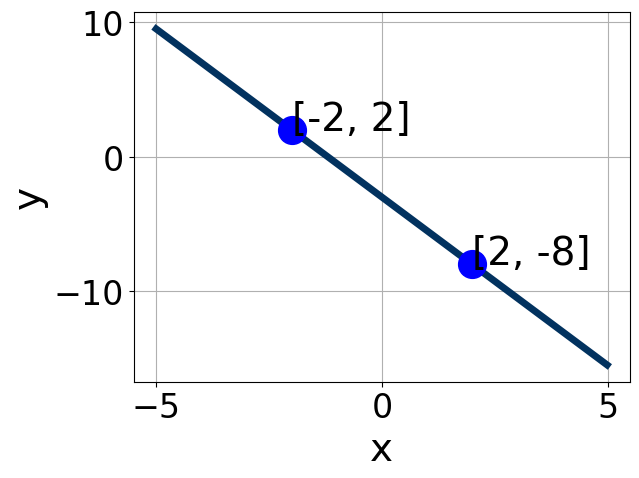
\includegraphics[width=0.5\textwidth]{../Figures/linearGraphToStandardC.png}
\end{center}
\begin{enumerate}[label=\Alph*.]
\item \( A \in [3, 5], \hspace{3mm} B \in [4.3, 6.84], \text{ and } \hspace{3mm} C \in [13, 17] \)
\item \( A \in [0.8, 1.8], \hspace{3mm} B \in [0.67, 1.34], \text{ and } \hspace{3mm} C \in [2, 7] \)
\item \( A \in [3, 5], \hspace{3mm} B \in [-5.94, -4.52], \text{ and } \hspace{3mm} C \in [-18, -5] \)
\item \( A \in [0.8, 1.8], \hspace{3mm} B \in [-1.22, -0.94], \text{ and } \hspace{3mm} C \in [-3, -2] \)
\item \( A \in [-6, 0], \hspace{3mm} B \in [-5.94, -4.52], \text{ and } \hspace{3mm} C \in [-18, -5] \)

\end{enumerate} }
\litem{
Find the equation of the line described below. Write the linear equation as $ y=mx+b $ and choose the intervals that contain $m$ and $b$.\[ \text{Perpendicular to } 7 x - 6 y = 15 \text{ and passing through the point } (-4, -9). \]\begin{enumerate}[label=\Alph*.]
\item \( m \in [-0.9, -0.61] \hspace*{3mm} b \in [-13.27, -12.32] \)
\item \( m \in [-0.9, -0.61] \hspace*{3mm} b \in [-5.44, -4.75] \)
\item \( m \in [0.71, 1.43] \hspace*{3mm} b \in [-6.03, -5.21] \)
\item \( m \in [-1.64, -1.14] \hspace*{3mm} b \in [-13.27, -12.32] \)
\item \( m \in [-0.9, -0.61] \hspace*{3mm} b \in [12.18, 13.19] \)

\end{enumerate} }
\litem{
First, find the equation of the line containing the two points below. Then, write the equation as $ y=mx+b $ and choose the intervals that contain $m$ and $b$.\[ (4, 3) \text{ and } (3, 10) \]\begin{enumerate}[label=\Alph*.]
\item \( m \in [-13, -3] \hspace*{3mm} b \in [2, 10] \)
\item \( m \in [-13, -3] \hspace*{3mm} b \in [-39, -26] \)
\item \( m \in [-13, -3] \hspace*{3mm} b \in [-3, 3] \)
\item \( m \in [7, 11] \hspace*{3mm} b \in [-12, -10] \)
\item \( m \in [-13, -3] \hspace*{3mm} b \in [31, 32] \)

\end{enumerate} }
\litem{
Solve the equation below. Then, choose the interval that contains the solution.\[ -13(2x + 6) = -14(8x -12) \]\begin{enumerate}[label=\Alph*.]
\item \( x \in [-1.13, -0.99] \)
\item \( x \in [-0.91, -0.68] \)
\item \( x \in [5.35, 5.78] \)
\item \( x \in [-4.5, -3.91] \)
\item \( \text{There are no real solutions.} \)

\end{enumerate} }
\litem{
\begin{enumerate}[label=\Alph*.]

\end{enumerate} }
\litem{
Solve the linear equation below. Then, choose the interval that contains the solution.\[ \frac{3x + 5}{4} - \frac{4x -7}{7} = \frac{6x -9}{5} \]\begin{enumerate}[label=\Alph*.]
\item \( x \in [-0.3, 1.2] \)
\item \( x \in [20.3, 22.3] \)
\item \( x \in [3.2, 4.2] \)
\item \( x \in [0.7, 2.7] \)
\item \( \text{There are no real solutions.} \)

\end{enumerate} }
\end{enumerate}

\end{document}